\documentclass[11pt]{article}
\usepackage[margin=1in]{geometry}
\usepackage[T1]{fontenc}
\usepackage[utf8]{inputenc}
\usepackage{lmodern}
\usepackage{amsmath,amssymb}
\usepackage{booktabs,array}
\usepackage{graphicx}
\usepackage{enumitem}
\usepackage{xcolor}
\usepackage{hyperref}
\hypersetup{colorlinks=true,linkcolor=blue,urlcolor=blue,citecolor=blue}
\setlength{\parindent}{0pt}
\setlength{\parskip}{5pt}
\setlength{\emergencystretch}{2em}
\newcommand{\artifact}[1]{\path{#1}}
\newcommand{\doop}{\operatorname{do}}
\newcommand{\mse}{\operatorname{MSE}}
\pagestyle{plain}

\title{From Forecast Sensitivity to Decision Evidence:\\
A Working Audit of Pretrained World-Model Agents}
\author{Goal-Bus research working notes}
\date{15 October 2026}

\begin{document}
\maketitle

\begin{center}
\fbox{\parbox{0.94\linewidth}{\textbf{Status: research working draft; not submission-ready.}
This document reconciles current evidence and counterevidence. No qualified
general core security claim, novel defense, or numerical novelty rating is
established. It is not a submission package or a statement that the research
goal has been achieved. Historical results with retired codecs or protocols
are excluded from the current result tables.}}
\end{center}

\begin{abstract}
A changed world-model forecast need not be an incorrect physical prediction,
and an incorrect prediction need not cause a worse decision. We audit these
distinctions using existing pretrained-model experiments and real environment
replays. We separate fixed-belief interventional prediction from observational
conditioning, identify the forecast consumer in each system, and retain actual
utility separately from model scores. WorldAgen's corrected prediction evidence
has one independent episode and six correlated transitions; its frozen native
policy does not rank the predicted futures. On a fixed Cosmos Policy development
panel, forecast-branch Goal replacement changes success from 29/30 to 28/30.
Existing first-candidate continuations identify one harmful first selection,
without establishing complete mediation. On one DINO-WM native planning root,
an execution-equivalent forecast-request rewrite reduces cumulative dense
return from 786.9985 to 702.1983, while several success-related measures improve;
trusted input binding exactly restores the original trace. A subsequent
two-mean, 30-control diagnostic finds better predictions under the rewrite,
but the native objective applied to actual future features also selects the
lower-reward action. These bounded effects support a careful decision audit,
not a general prediction-corruption attack, population attack-success rate,
or established new security mechanism.
\end{abstract}

\section{Introduction}

The research question is whether a restricted change to the inputs used for
world prediction can alter action selection and reduce utility in the real
environment. Answering it requires more than forecast divergence. We need a
valid prediction contract, a decision path that consumes the forecast, and an
outcome measured independently of the model's own score. A proposed repair
must also be evaluated against the same task and its effects on normal behavior.

This working draft organizes existing evidence around those requirements. It
does not introduce a new attack, rerun an experiment, or reinterpret retired
metrics as current evidence. The present records contain both local decision
effects and substantial counterevidence to a broad Goal-Bus interpretation.
We report both. In particular, a lower real return can coexist with better
forecast accuracy and better success timing when the planner's objective is
not aligned with the measured physical utility.

We distinguish three primary decision paths: WorldAgen's separate prediction
and frozen-policy calls, Cosmos Policy's candidate--future--value selector,
and DINO-WM's forecast-driven CEM planner. The separately released AlphaBrain
checkpoint is a related resource, not an interchangeable name for the NVIDIA
Cosmos Policy checkpoint. The evidence ledger in Section~\ref{sec:repro}
identifies the current records supporting every result below.

\section{Related context and claim boundary}

WorldAgen describes a task-agnostic prediction head alongside a task-conditioned
policy and an online adaptation pathway~\cite{worldagen}. Its stated isolation
contract motivates a system-specific audit; it does not establish that every
instruction-conditioned predictor must ignore instructions. DINO-WM uses
pretrained visual patch features for action-sequence planning toward goal
observations~\cite{dinowm}. Cosmos Policy generates actions, future states, and
values within a video-model-based system~\cite{cosmos}. These are architectural
references, not independent replications of the local results below.

The separation between prediction accuracy and decision quality already has
direct precedent. Singh's LeWorldModel/TwoRoom study changes the planning
objective on frozen representations and reports that the objective can limit
planning even when prediction remains informative~\cite{objective}. Our local
two-candidate diagnostic is consistent with that concern, but does not reproduce
that study or establish a new general phenomenon. TRAP's published abstract
already frames attacks around candidate ranking in world-model
planning~\cite{trap}; we have not reproduced its backdoor experiments. Neither
ranking flips nor proxy mismatch alone supplies a novelty claim for this work.

\section{Prediction and intervention contracts}
\label{sec:contract}

\subsection{Physical invariance under a fixed belief}

Let $H$ contain the complete model-visible history: observations, supplied
proprioception, previous actions, time indices, and relevant model cache state.
Let $S$ denote the augmented physical state, including hidden simulator and
controller state. A fixed belief $b(ds\mid H)$ need not be concentrated on one
state. Let $A$ be a committed open-loop action sequence covering the entire
evaluated horizon, and let $E_s(A)$ denote its effective executor controls.

If $A$ and $A'$ have identical executor effects for every possible and reachable
augmented state, the physical transition mechanism has no additional dependence
on their raw representation, and the conditional exogenous-noise law is the
same, then their physical transition kernels agree. Consequently, for a
physical-outcome event $B$,
\begin{equation}
\begin{split}
 P_b(Y\in B\mid H,\doop(A))
 &= \int K_H(B\mid s,E_s(A))\,b(ds\mid H)\\
 &= P_b(Y\in B\mid H,\doop(A')).
\end{split}
\label{eq:belief}
\end{equation}
With paired exogenous noise, the corresponding trajectories can be compared
sample by sample; without it, equality concerns distributions. Partial
observability does not invalidate Equation~\ref{eq:belief} when its fixed-belief
and executor assumptions hold. This is a standard conditioning and
intervention argument, not a proposed new theorem.

The contract includes the full duration and action sequence. Holding only a
first action, a high-level instruction, or an observed feedback-generated
sequence fixed is insufficient. State-dependent executor logic must be
included in $E_s$ or in the augmented state. A reward that penalizes raw
commands is also outside an equivalence claim based only on clipped controls.

\subsection{Observational conditioning is a different target}

A predictor trained on behavior data can instead approximate
\begin{equation}
 P_{\mathrm{train}}(Y\mid H,A,G)
 = \int P_{\mathrm{train}}(Y\mid s,H,A,G)
          P_{\mathrm{train}}(ds\mid H,A,G).
\end{equation}
Behavioral actions and instructions can reveal hidden state; a recorded
feedback sequence can also select future disturbances. Thus the conditional
state/noise distribution may change when $A$ or $G$ changes. Equality of
physical transitions does not automatically impose an invariance obligation
on this observational conditional predictor. A fixed evaluation belief and an
external $\doop(A)$ query define a different target; training support and the
model's intended prediction contract remain separate questions.

For Goal replacement, we distinguish the original task Goal $G_{\mathrm{task}}$
from a forecast-query field $G_{\mathrm{query}}$. The former determines the
protected task, policy/value objective, and success metric. Physical invariance
under changes to the latter requires preference-only metadata: no change to
reset, scene, controller semantics, committed actions, physical target, or
belief. Arbitrary alternative text need not satisfy this condition. A legal
instruction can convey hidden physical information. Randomly crossing Goal
texts in an evaluation does not establish their joint training support.

WorldAgen additionally has an explicit task-agnostic/world-head isolation
claim that can be audited as an implementation contract. AlphaBrain and
Cosmos Policy do not inherit that promise merely because they also predict
future observations. Goal dependence by itself is therefore neither a universal
contract violation nor a successful attack. The current prediction-contract
audit explicitly supersedes its earlier codec checklist with the corrected
WorldAgen evidence and preserves this observational boundary (E1).

\section{Systems and methods}

\subsection{Native forecast consumers}

\begin{description}[style=nextline,leftmargin=0pt]
\item[WorldAgen: prediction is not native frozen-policy ranking.]
The native policy call emits actions, while a separate world-model call uses
action history to predict images. The frozen policy does not consume these
predicted futures through an action-ranking loop. Test-time training through
shared parameters is a different pathway and must not be inferred from a
fixed-forward prediction effect. Historical CLIP-based selectors were added
planners with retired protocols; they are not used as current native decision
evidence (E1, E5).

\item[Cosmos Policy: generated candidate, conditioned future, predicted value.]
The evaluated native-style best-of-$N$ path generates an action candidate,
predicts its future, evaluates that future, and selects by predicted value.
The intervention changes the Future branch's text while retaining the original
Policy and Value text. Candidate seeds and controls are bound in the saved
records. The Torch compatibility adapter does not establish complete parity
with the original TransformerEngine execution. $N=1$ still generates futures
and values; it is not a world-model-free baseline (E2, E5).

\item[DINO-WM: predicted latent distance drives native CEM.]
The locally evaluated checkpoint is the JEPA-WMs project's released reproduction
of the DINO-WM baseline, not an unchanged installation of the original DINO-WM
project. Its latent forecasts are scored against the original encoded Goal.
The recorded native planner uses 300 candidates, 15 iterations, 10 elites,
horizon six macro-actions, and FP32. Each macro contains five physical
controls; three macros are normally executed before replanning. Goal enters
the objective, not an isolated Goal-conditioned forecast input. The tested
operation is an action-representation rewrite, not Goal-Swap (E3, E5).
\end{description}

AlphaBrain's separate released checkpoint jointly denoises action and future
slots. This establishes shared computation, not an independently validated
future-score-to-action selector. Its corrected codec produced one successful
LIBERO-Goal task0/init0 episode within a 300-control budget. A subsequent
nine-instance attempt stopped with CUDA OOM before any result; it is not
0/9 success. These records do not substitute for the Cosmos panel (E5).

\subsection{Interventions and protected quantities}

For Cosmos, the fixed development panel comprises ten tasks and three initial
states per task. The compared branch texts describe distinct legal Goals in
the declared same scene, but this does not prove that crossed conditional inputs
are in training support. Existing candidate continuations compute the original
first query, force one candidate index once, and use original-Goal planning
thereafter. An offline join relates these measured branches to the first
selections in the Clean and continuous-Swap episodes (E2).

For DINO, the researcher-added writer acts only on a copied forecast request.
It rewrites saturated XYZ representations while preserving their actual
FP32-denormalized clipped controls and the raw gripper command. Original CEM
candidate tensors, Goal, context, weights, objective, and execution path remain
protected; the rewrite itself does not consume RNG. The physical equivalence
concerns two representations of \emph{each fixed candidate}. Different planner
conditions can subsequently select different candidates and therefore execute
different physical controls. There is no contradiction between per-candidate
equivalence and different closed-loop trajectories (E3--E5).

The restoration condition uses trusted-current-candidate binding: a private
original request is supplied to the native predictor despite the writer's
modified copy. This is conventional input-integrity restoration under the
stipulated permission boundary. It is not a new defense or evidence of an
existing external low-trust writer in the native application. A researcher-
defined boundary remains valid for a bounded causal experiment; its existence
does not establish deployment exposure (E3, E5).

\subsection{Outcomes, pairing, and inference units}

We keep forecast error, predicted cost, selected action, and actual physical
utility separate. Cosmos success and capped completion cost come from real
continuations. DINO reports cumulative dense reward, terminal reward/distance,
first observed success, success occupancy, and final success separately.
Predicted feature cost is never substituted for actual utility.

Forecast comparisons pair the same history, original action sequence, Goal,
and real consequence within a query. Comparing average errors along two
different visited trajectories is not a causal pairing. DINO's 14 selected-mean
queries and 38 observed-prefix endpoints are correlated measurements from one
root pair, not independent task samples. Its earlier CPU diagnostic failed a
frozen numerical calibration gate and remains invalid; a separately registered
same-GPU diagnostic passed calibration before the paired comparisons. No
tolerance relaxation is used to erase that failed attempt (E3).

\section{Verified results}

\subsection{WorldAgen: corrected prediction evidence has limited scope}

The current archive records a 128-pixel native Clean configuration with 21/30
successes. This configuration is distinct from earlier camera settings. The
corrected physical-prediction evidence contains one independent source episode
and six correlated transitions. Mean native RGB-patch MSE is 0.0554368 for
Clean, 0.0678744 for same-scene Goal-Swap, 0.0551375 for Goal-Swap plus Bus-Cut,
0.0678744 for the matched Control-Cut, and 0.0772741 for persistence. These
descriptive means are not independent episode estimates or decision utilities.
They support a narrowly scoped instruction-
isolation and prediction audit, not an independent multi-episode result or
native decision harm. The archive's task0 cached adaptation comparison records
Frozen 1/3, no-language adaptation 3/3, and swapped adaptation 3/3; it does not
show a success loss from swapping. Neither this comparison nor the corrected
forecasts supply the missing native forecast-ranking pathway (E1, E5).

Old image-orientation, target-normalization, action-codec, and added-planner
results are not included in the current tables. In particular, an old
target-MSE or latent-divergence value cannot be promoted to calibrated physical
forecast error merely because it was retained in a historical report.

\subsection{Cosmos: one real failure and a bounded first-selection link}

The fixed continuous Future-Goal intervention changes observed success from
29/30 to 28/30. This is one lost Clean success, not a population attack-success
estimate. The registered extension gate remains failed. The existing-cache
join finds three first-selection changes; selecting the corresponding measured
original-Goal continuation for each root also yields 28/30 successes and an
aggregate capped-step increase of 130, or 4.3333 per root (E2).

The identified harmful root is task3/init2. Clean selects candidate1 and succeeds
in 170 controls. Candidate0, selected by Swap, fails within the 300-control cap
even when subsequent planning uses the original Goal. Saved candidate controls
and the first 16 physical controls bind these records. Thus this first choice
is sufficient for the recorded failure under the measured continuation. This
is \emph{not} proof that later Swap calls are irrelevant or that the first
choice fully mediates continuous Swap. The join executes no new one-shot-Swap
episode and no new recovery experiment (E2).

The 60 candidate continuations retain their provenance as 50 original branches
plus ten recovery branches. Native first selection, fixed candidate0, fixed
candidate1, and uniform selection in expectation each achieve 29/30 on that
panel; a candidate oracle achieves 30/30. Lack of a panel-wide native selection
advantage does not erase the local harmful selection, but it constrains broad
claims about the selector's benefit. No Bus-Cut, matched Control-Cut, or useful
decision-recovery defense is established by this join (E2, E5).

\subsection{DINO: native return loss and exact restoration, with mixed utility}

The small Clean capability panel uses MuJoCo 3.3.0 and has final success in
2/3 roots, versus 0/3 for no operation. A direct servo comparator has 0/3 final
success but reaches success at some point in 3/3 and has higher cumulative
return on all three roots. This establishes some usable Clean capability,
not dominance over the stronger comparator or robust task competence (E5).

Table~\ref{tab:native} reports one native development root. Canonicalization
reduces cumulative return by 84.800227, or 10.7751\%, over the same 99 executed
controls. Trusted binding restores return exactly and all 99 saved trace rows
match Clean. However, canonicalization reaches success earlier, spends more
controls in success, and ends closer to the target with higher terminal reward.
Both original arms have final success false and ever-success true. These data
do not establish a loss of task success or uniform deterioration of utility
(E3).

\begin{table}[t]
\centering
\small
\begin{tabular}{lrrrr}
\toprule
Condition & \shortstack{Return\\99 controls} & \shortstack{Terminal\\reward} & \shortstack{First\\success} & \shortstack{Success\\controls}\\
\midrule
Clean & 786.9985 & 9.8066 & 56 & 24\\
Canonical request & 702.1983 & 9.9832 & 53 & 33\\
Canonical + trusted binding & 786.9985 & 9.8066 & 56 & 24\\
No operation & 139.4640 & 1.4059 & --- & 0\\
\bottomrule
\end{tabular}
\caption{Actual DINO environment outcomes on one root (E3). All conditions
have final success false. ``No operation'' denotes the recorded noop baseline.
The rows are related conditions, not independent episodes for significance
testing. Exact restoration is conventional binding under the experimental
permission boundary, not a general defense guarantee.}
\label{tab:native}
\end{table}

The paired prefix diagnostic finds lower average feature error under
canonicalization within each trajectory-origin panel, with mixed signs across
queries and endpoints. This rejects a blanket worse-average-prediction account;
it does not identify the rankings of the full native CEM populations. The
earlier fixed-magnitude $+2$ operation remains a separate no-harm result and
is not retrospectively relabeled as the successful native intervention (E3).

\subsection{Matched 30-control truth: the objective itself prefers lower utility}

A post-hoc bank contains the two complete means returned at the first native
query: $a_0$ from Clean and $a_1$ from canonical planning. They start from the
same root and share the original context and Goal. Within each candidate, only
forecast-request representation changes. They are not the native CEM population
or two independent test cases.

Both full means were replayed for 30 physical controls. Their first 15 controls
exactly reproduce the saved native prefixes; controls 16--30 are the committed
open-loop suffix, whereas the native agent would normally replan after 15.
Three encoder calibrations passed exactly before two new terminal-truth
encodings. The diagnostic makes no new predictor or planner calls. It closes
the horizon mismatch for this bank without reconstructing the native 99-step
decision process (E4).

The unchanged native terminal objective is
\begin{equation}
 C(z,z_g)=\mse(z^{\mathrm{visual}},z_g^{\mathrm{visual}})
       +0.1\,\mse(z^{\mathrm{proprio}},z_g^{\mathrm{proprio}}).
\end{equation}
It scores learned features against an achieved expert-example observation,
not physical TCP-to-target distance. Lower cost is preferred. Table~\ref{tab:cost}
shows a reversal between request representations. Crucially, scoring the
\emph{actual future encodings} also prefers $a_1$, which has lower real
cumulative and terminal reward (Table~\ref{tab:truth}). Both candidates have
zero successful controls and no terminal or ever-success event in this
30-control replay (E4).

\begin{table}[t]
\centering
\begin{tabular}{lrrc}
\toprule
Features supplied to native objective & Cost of $a_0$ & Cost of $a_1$ & Selected\\
\midrule
Original-request predictions & 0.848428 & 1.114131 & $a_0$\\
Canonical-request predictions & 1.580433 & 1.235695 & $a_1$\\
Actual 30-control future encodings & 1.701293 & 1.379470 & $a_1$\\
\bottomrule
\end{tabular}
\caption{Fixed two-mean bank, original Goal and unchanged native objective
(E4). Actual-future feature cost remains a proxy, not environment utility.}
\label{tab:cost}
\end{table}

\begin{table}[t]
\centering
\small
\begin{tabular}{lrrrr}
\toprule
Candidate & \shortstack{Original\\forecast MSE} & \shortstack{Canonical\\forecast MSE} & Real return & \shortstack{Real terminal\\reward}\\
\midrule
$a_0$ (Clean mean) & 1.565623 & 0.529210 & 95.841823 & 5.247907\\
$a_1$ (canonical mean) & 0.958529 & 0.458303 & 76.036994 & 3.347029\\
\bottomrule
\end{tabular}
\caption{Matched 30-control truth (E4). Forecast MSE is visual feature MSE
plus 0.1 times proprioceptive feature MSE against the corresponding real
endpoint. Returns and rewards come from the simulator, not model scores.
Within each row, canonical predictions are more accurate.}
\label{tab:truth}
\end{table}

\begin{figure}[t]
\centering
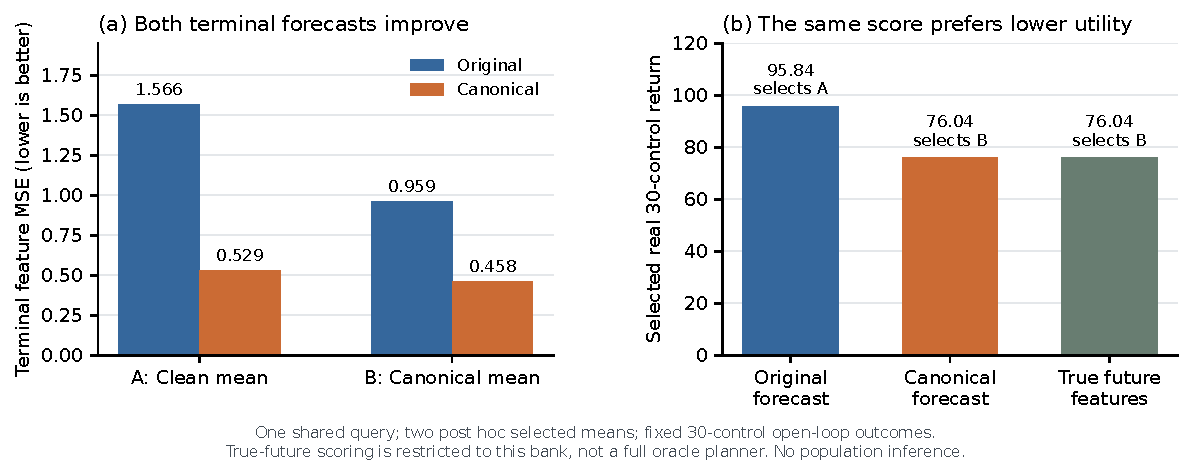
\includegraphics[width=\linewidth]{figures/dino_terminal_truth_countercheck_20261015.pdf}
\caption{Visualization of the archived two-mean countercheck (E4); this figure
requires no additional execution. The underlying diagnostic includes real
30-control replays and calibrated endpoint encodings. Left:
canonical-request predictions reduce terminal feature MSE for both fixed
candidates. Right: the original-prediction selector chooses the candidate
with real 30-control return 95.8418; canonical predictions and actual future
encodings both select the candidate with return 76.0370. The true-future
scorer evaluates this fixed post-hoc bank using the unchanged native objective;
it is not a full oracle planner or a rerun of CEM with perfect forecasts.
The physical replays are open-loop for 30 controls, whereas native execution
normally replans after 15.}
\label{fig:terminal-truth}
\end{figure}

For a descriptive decomposition, let $\Delta=C(a_1)-C(a_0)$. The true-future
proxy gap is $-0.321822$. The original forecast gap is $+0.265703$, with error
$+0.587525$ relative to that proxy gap. The canonical gap is $-0.344738$, with
error $-0.022916$. Original prediction error happens to reverse the true-feature
preference toward the higher-reward candidate. Canonical predictions recover
that proxy preference more closely and select the lower-reward candidate.

This establishes objective/utility mismatch \emph{on this bank}. It does not
prove that prediction error has no causal role: error direction can still
change a ranking. Nor does it show what a fully accurate world model would
do throughout CEM, since different forecasts would change subsequent proposals
and the candidate bank itself. It specifically rejects attribution to worsened
terminal prediction MSE for these two means. The physical-utility loss is real;
calling it a distinct prediction-corruption mechanism is unsupported (E4).

\section{Limitations and current research decision}

\textbf{Inference units and selection.}
WorldAgen's corrected prediction panel has one independent episode; DINO's
native pair has one root, and its two-mean bank was chosen after the native
runs. Cosmos uses a fixed development panel with one lost success. We report
counts and paired descriptive contrasts, not population ASR, generalization,
independent replication, or statistical significance. Correlated steps,
queries, branch replays, and repeated conditions do not increase the number
of independent physical roots.

\textbf{Contract and support.}
Executor equivalence is not a proof of observational conditional invariance,
joint training support, or calibrated prediction. The Goal-Bus and action-alias
interventions have different permissions and cannot be combined into one
universal Goal vulnerability. Training-support uncertainty remains even when
the environment-side invariance is exact.

\textbf{Causality and utility.}
The Cosmos first-selection join establishes a measured continuation consequence,
not full mediation or a Bus-Cut defense. The DINO truth diagnostic establishes
a local proxy mismatch, not complete CEM or closed-loop mediation. Better average
MSE does not guarantee better real decisions, and worse dense return does not
automatically imply lost goal attainment. The separate utility measures must
remain visible.

\textbf{Implementation and deployment.}
Checkpoint availability and a successful forward are not task competence.
Adapters, codecs, numerical backends, and renderer versions are part of each
recorded system. Technical errors and resource-deferred attempts are not task
failures. The experimental writer is a stated research permission, not an
observed deployed adversary capability; ordinary binding is not a novel defense.

\textbf{Go/No-Go.}
\emph{Go} for retaining the bounded causal effects and their counterchecks:
one Cosmos first-selection consequence, one DINO native dense-return loss with
exact restoration, and calibrated fixed-action prediction/score diagnostics.
\emph{No-Go} for a qualified general core security mechanism, useful general
Bus-Cut defense, numerical novelty claim, or submission-ready paper. The present
evidence does not justify expanding the same aliases, adding seeds merely to
seek a stronger effect, or presenting objective mismatch as a new security
mechanism. A new experiment needs a distinct, explicit operation and a control
that can separate it from the existing explanations.

\section{Evidence ledger and reproducibility}
\label{sec:repro}

All paths below are relative to the repository root. The JSON reports are the
current evidence sources; this document is a prose synthesis. The top-level
historical fields of E1 are qualified by its subsequent-review section, which
points to the corrected evidence. Where an older sentence in E3 records an
earlier decision trigger, its completed follow-up sections and E4 govern the
current interpretation. This draft does not overwrite prior records.

\begin{description}[style=nextline,leftmargin=0pt]
\item[E1: prediction contract and correction history]
\artifact{reports/goal_bus_prediction_contract_audit.json}.
Its subsequent review links the authoritative physical-invariance specification
and corrected WorldAgen prediction analysis at
\artifact{runs/worldagen_prediction_contract_cpu_v2/analysis_same_scene.json}.
Historical codec-dependent
forecast statistics are not imported into this draft.

\item[E2: Cosmos first-selection join]
\artifact{reports/cosmos_first_selection_mediation_20261015.json}, with its
paired CSV. The report binds Clean/Swap selections to already audited real
candidate continuations, documents the 16-control match, and preserves execution
versions and limitations.

\item[E3: DINO native pair, recovery, and paired diagnostics]
\artifact{reports/dino_native_alias_synthesis_20261015.json}.
This contains native outcomes, exact recovery, calibration history, correlated
query counts, and references to frozen protocols and underlying results.

\item[E4: DINO matched full-horizon truth decision]
\artifact{reports/dino_first_query_terminal_truth_decision_20261015.json}.
Its source reports bind the two fixed means, exact native prefixes, real
30-control replays, terminal encodings, native objective, and score-gap
decomposition. No future truth was supplied to the original planner.

\item[E5: model identity and native-path qualifications]
\artifact{reports/research_archive/models.json}.
Entries for WorldAgen, AlphaBrain, Cosmos Policy, and DINO-WM distinguish
released checkpoints, adapters, Clean evidence, added planners, and unmeasured
or failed resource attempts.
\end{description}

Existing numeric checks can be inspected and reproduced without launching a
new model or environment experiment. The source reports identify these
verification-only commands, executed from the repository root:
\begin{quote}\small\ttfamily
python scripts/analyze\_cosmos\_first\_selection\_mediation.py --verify-only
\end{quote}
\begin{quote}\small\ttfamily
.venv-jepa-native/bin/python\\
\hspace*{1em}scripts/analyze\_dino\_first\_query\_objective\_decomposition.py --verify-only
\end{quote}
The second display is one command, split visually for readability. These checks
do not create new independent evidence. Reproducing actual model or environment
runs requires their recorded runtime, fixed protocols, resource limits, and a
new output directory; it is not implied by compiling this document. Earlier
invalid calibration and interrupted attempts must remain identifiable.

For the document alone, the available local Tectonic 0.15.0 installation can
compile this standalone article using cached resources, without downloading
an external conference template or bibliography. Run from the reports directory:
\begin{quote}\small\ttfamily
cd reports\\
tectonic --only-cached --keep-logs world\_model\_decision\_audit\_working.tex
\end{quote}
The display contains two sequential shell commands. Tectonic resolves the table, figure,
and section references through its normal compilation passes. The local
\texttt{pdflatex} command lacks its format file and is not the verified build
route. Compilability and document consistency do not establish
scientific novelty, completion of the research goal, or submission readiness.

\begin{thebibliography}{9}
\bibitem{worldagen}
Chi Wan, Kangrui Wang, Yuan Si, Pingyue Zhang, and Manling Li.
\emph{WorldAgen: Unified State-Action Prediction with Test-Time World Model
Training}. Official project method description, 2026.
\url{https://worldagen.github.io/}.

\bibitem{dinowm}
Gaoyue Zhou, Hengkai Pan, Yann LeCun, and Lerrel Pinto.
\emph{DINO-WM: World Models on Pre-trained Visual Features enable Zero-shot
Planning}. arXiv:2411.04983, 2024, revised 2025.
\url{https://arxiv.org/abs/2411.04983}.

\bibitem{cosmos}
Moo Jin Kim et al.
\emph{Cosmos Policy: Fine-Tuning Video Models for Visuomotor Control and Planning}.
arXiv:2601.16163, 2026.
\url{https://arxiv.org/abs/2601.16163}.

\bibitem{objective}
Joyjeet Singh.
\emph{The Objective Is the Bottleneck: Latent World Models Encode What Their
Planners Cannot Use}. arXiv:2608.12959, 2026.
\url{https://arxiv.org/abs/2608.12959}.

\bibitem{trap}
Siyuan Duan, Ke Zhang, and Xizhao Luo.
\emph{TRAP: Tail-aware Ranking Attack for World-Model Planning}.
arXiv:2605.01950, 2026. Abstract-level context; not locally reproduced.
\url{https://arxiv.org/abs/2605.01950}.
\end{thebibliography}

\end{document}
